% Template for ICME 2018 paper; to be used with:
%          spconf.sty  - ICASSP/ICIP/ICME LaTeX style file, and
%          IEEEbib.bst - IEEE bibliography style file.
% --------------------------------------------------------------------------
\documentclass{article}
\usepackage{spconf,amsmath,epsfig}

\pagestyle{empty}
\usepackage{color}

\newcommand{\comments}[1]{}
\newcommand{\xj}[1]{\textcolor{red}{(xuejin: #1)}}
\newcommand{\change}[1]{\textcolor{blue}{#1}}
\newcommand{\vb}[1]{\mathbf{#1}}


\begin{document}\sloppy

% Example definitions.
% --------------------
\def\x{{\mathbf x}}
\def\L{{\cal L}}


% Title.
% ------
%\title{ACCURATE SEGMENTATION OF SYNAPTIC CLEARANCE WITH DEEP CONVOLUTIONAL NETWORKS AND A NOVEL CONTOUR GROWING ALGORITHM}
\title{Accurate Segmentation of Synaptic Clearance with post contour growing conjuncated with a ConvNet}
%
% Single address.
% ---------------
\name{Paper 1378}
\address{}


\maketitle


%
\begin{abstract}

Synaptic cleft is an important area for neuroscientists to analyze the macromolecular complexes related to neurotransmitter transmission.
However, the large amount of noise and low signal-to-noise ratio in raw electron micrographs make it significantly challenging to extract this region automatically.
%
In this paper, we propose a simple but effective framework to automatically extract accurate boundaries of synaptic cleft regions.
Our approach concatenates a contour growing step to a fully convolutional network (FCN), so that it takes the advantage of large receptive fields of FCNs to precisely localize the synaptic cleft region in a noisy image, and then extract the region boundaries by a fine-level contour evolution technique.
%
While considering both the texture and contours, our approach is more robust to noises, and outperforms all existing single-model FCNs on accurate segmentation of synaptic clefts in electron micrographs.

 
\end{abstract}
%
\begin{keywords}
Synaptic clef extraction, fully convolutional networks, active contours, contour growing
\end{keywords}
%
%%%%%%%%% BODY TEXT
\section{Introduction}
\label{sec:intro}
Electron micrographs (Fig.~\ref{fig:img} (a)) are obtained by cryo-electron tomography (CET) \cite{Hawkes2007}, which is an advanced technique to visualize the \change{near-to-native} environment of neurones, such as cytosol or lysate and lipid membranes~\cite{Lucic2005a}.
\xj{I can not find anyone using "near-to-native". you use 'native' many times in the draft.}
%
Among all kinds of cellular materials, biological macromolecules in synaptic cleft regions are one of the hottest study areas, as they play an important role in neurotransmitter transmission.
%
In the last decade, it mainly relied on manual segmentation of synaptic cleft regions, which is time-consuming and subjective, to analyze those macromolecules of interest.
%
Our goal in this paper is to develop an automatic approach to automatically extract the accurate region of synaptic cleft from noisy electron micrographs (Fig.~\ref{fig:img} (b)).


%The challenges behind this task are not easy to resolve by existing segmentation methods.
Automatic segmentation of synaptic cleft is challenging in many aspects. 
Firstly, due to the radiation damaging during CET, electron micrographs suffer from a large amount of noise and low signal-to-noise ratio (SNR).
Secondly, the synaptic cleft region is typically a quite small fraction of a high-resolution $2D$ electron micrograph, which requires a high precision of segmenting small objects.
Thirdly, only the cellular cleft, adjacent to one synapse and receiving neurotransmitter molecules from another synapse, is the desired synaptic cleft. This requires the segmentation technique to encode munch \xj{much more global?} biological knowledge for judgement.
Finally, as the most of concerned macromolecules exist on the surface of presynaptic membranes, it puts forward a higher demand on accurate contour localization.

\begin{figure}[t]
    \begin{center}
        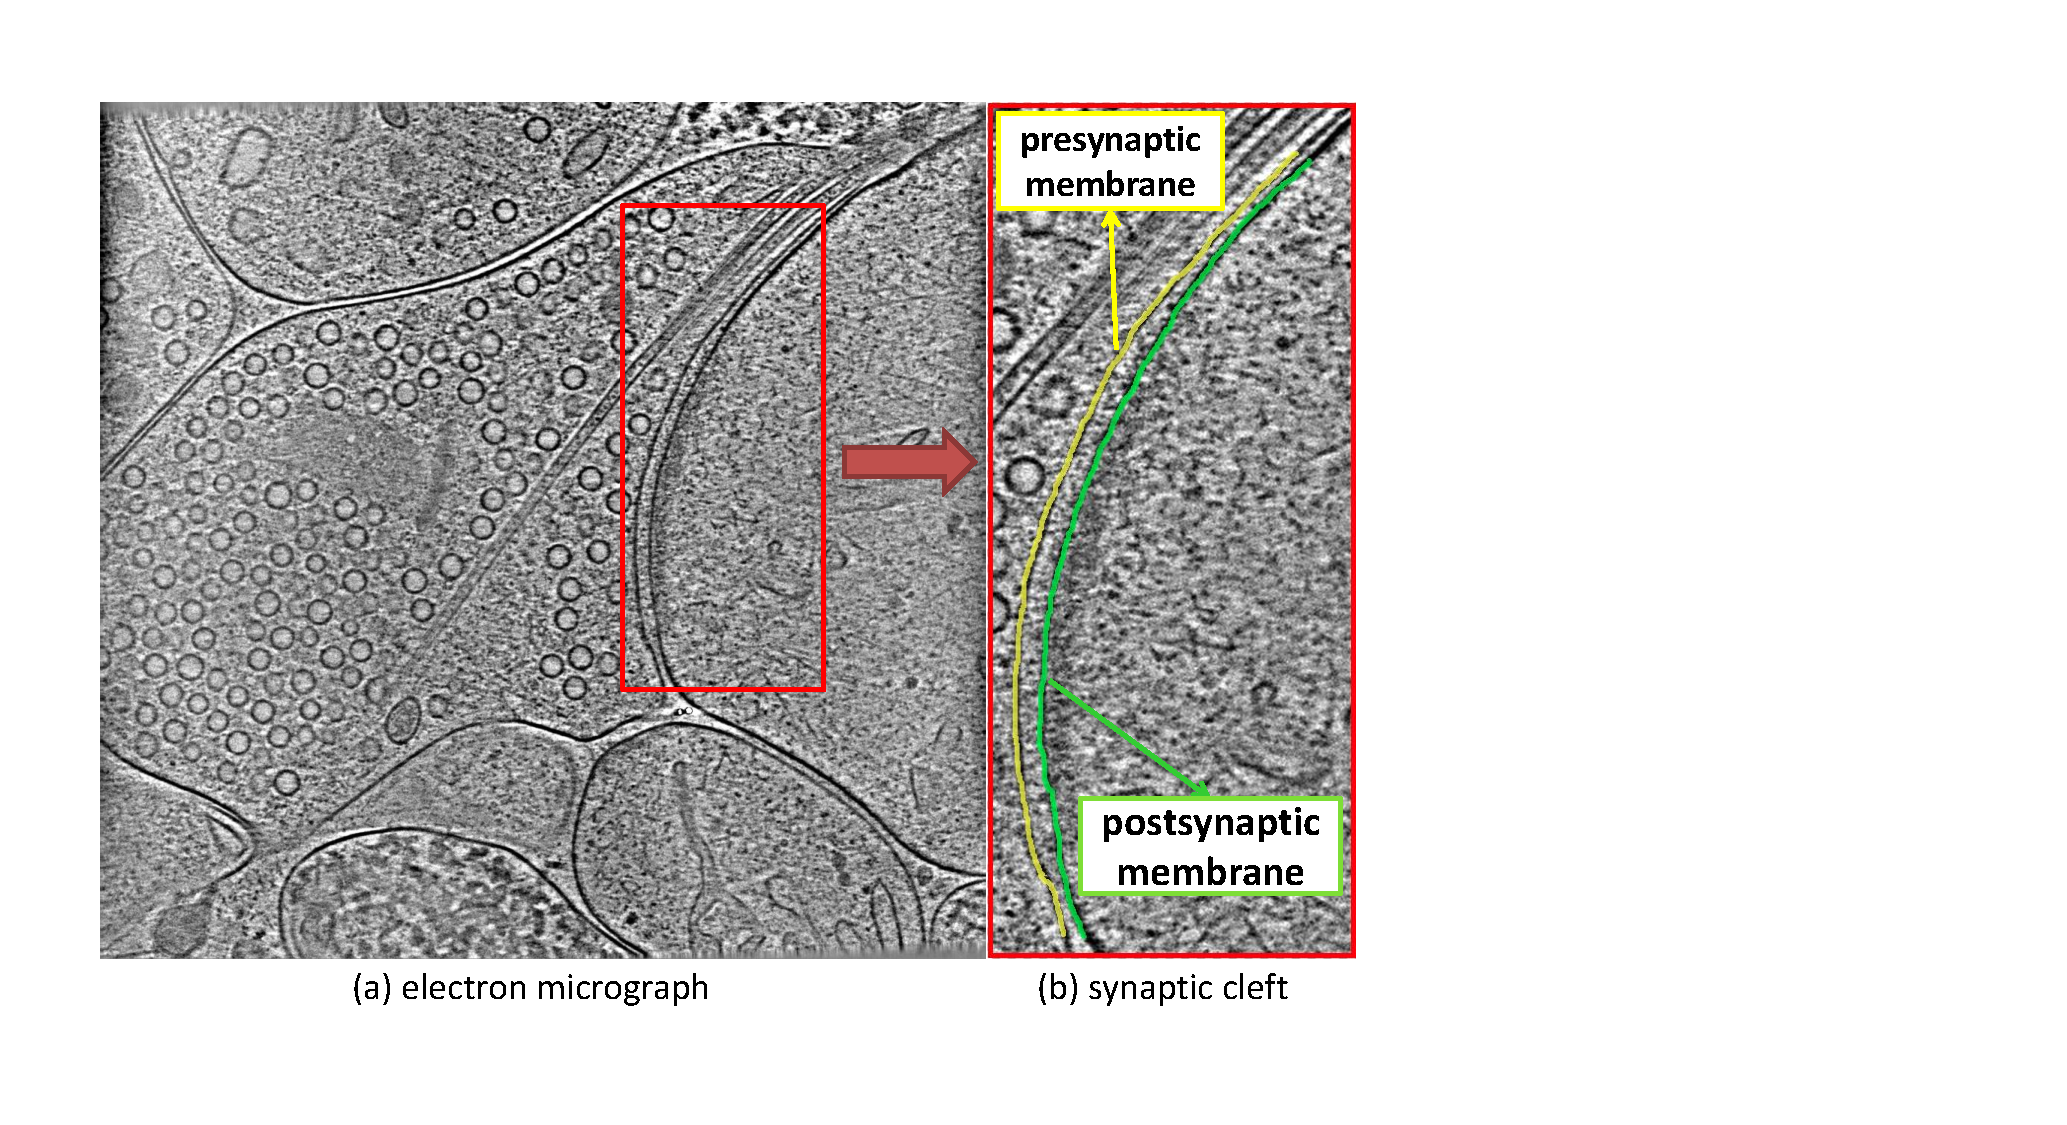
\includegraphics[width=3.4in]{figs/FigImg.pdf}
   \end{center}
\caption{(a) An electron micrograph containing a synaptic cleft region in the red box. 
            (b) Especially, the synaptic cleft region is surrounded by a presynaptic membrane (yellow) and a postsynaptic membrane (green). \xj{emphasize the region with a mask?} }
\label{fig:img}
\end{figure}


Recently, fully convolutional networks (FCN)~\cite{Long2015,Ronneberger2015,Chen2016a,Chen2017,Zhao2016} have achieved great progress in image segmentation, and variants of FCN \cite{Ronneberger2015,Chen2017,Dhungel2015,Lieman-Sifry2017,Chen2016b,Ourselin} show their promising performance in biomedical image processing.
%
The famous U-net~\cite{Ronneberger2015} directly concatenates the features from downsampling to upsampling layers for supplementing low-level information and better contour localization.
Soon, Chen et al.~\cite{Chen2016a} developed the dilated convolution operation by introducing zeros into the original convolutional kernel for lager receptive field and achieved amazing performance in natural image segmentation.
DCAN~\cite{Chen2017} integrates complementary information of objects and contours in a multi-task learning framework to separate the clustered objects into individual ones.
Moreover, PSPNet~\cite{Zhao2016} uses the more powerful ResNet~\cite{He2016} for feature extracting and proposes a pyramid pooling module to better exploit the global context information.
%
Although these techniques have achieved great success in many challenging datasets, they still face challenges when processing electron micrographs, which have unique textures and structures.

\xj{For referennces, use author [ref] proposed a method... or A method is proposed [ref] to ...}

\begin{figure*}[t]
    \begin{center}
        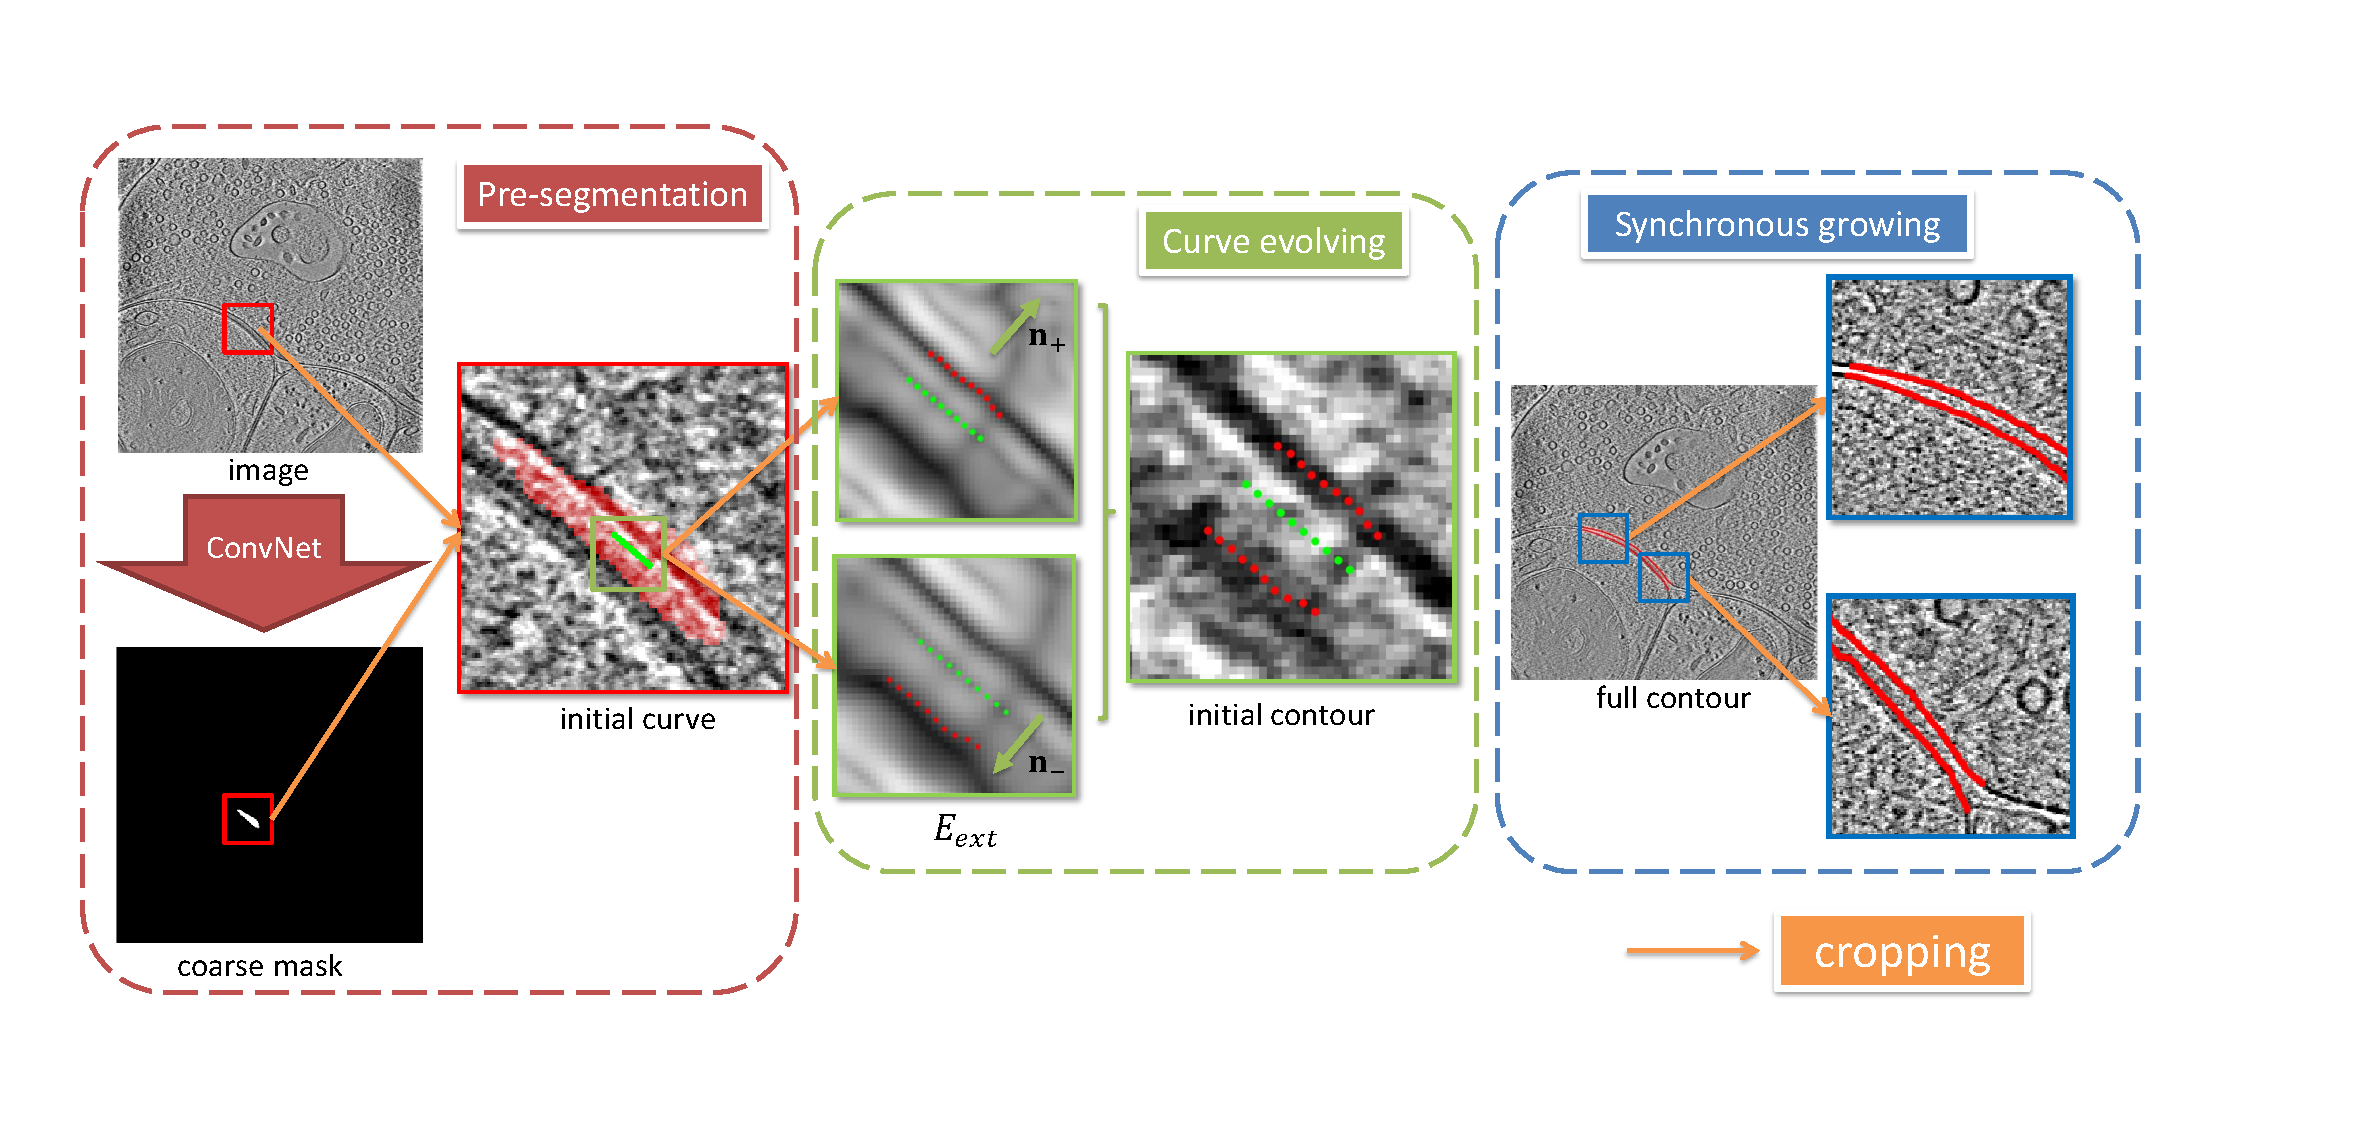
\includegraphics[width=7in]{figs/FigCG.pdf}
   \end{center}
\caption{A brief view of our algorithm in localizing the synaptic cleft region. First a CNN-based model results in a coarse segmentation mask, which provides an initial curve (green line) in cleft region.
        Then, the initial curve is respectively evolved along opposite direction ($\mathbf{n}_+$ and $\mathbf{n}_-$) to obtain two pieces of initial contours (red dotted line).
        Finally, the two contours will synchronously grow to localize the whole synaptic cleft region (encircled by red solid curves).}
\label{fig:cg}
\end{figure*}


Though FCNs have difficulties on extracting precise boundaries for synaptic cleft, our method is built on FCNs, taking their advantages of efficiently localizing the synaptic cleft region in a large-size electron micrograph. 
%
Then a novel contour growing process is concatenated to the FCN to extract accurate contours of the target synaptic cleft region.
%

\comments{
In this paper, we propose an effective framework for segmenting target region in electron micrographs by combining intelligent CNN \xj{{better using FCN?}} and a novel contour growing algorithm.
Our method consists of two main steps.
First, a FCN-based segmentation is employed to coarsely extract the synaptic cleft region. \xj{only one cleft region or mulitple regions?}
%
And then, our contour growing algorithm takes in the segmentation and results in precise contour localizations of target synaptic cleft region.}
The insight of our method is that the contours localized by FCNs are usually poor and unsatisfied, due to successive downsampling layers~\cite{Chen2017}, but it successfully produces an accurate localization of our plausible region.
%
Therefore, we utilize the ability of FCN of learning high-level biological knowledge to globally pick out synaptic cleft regions from such a complex environment.
%

Our contour growing algorithm is robust and efficient, because it is a self-correcting model and uses the local texture information for inference.
With a coarse segmentation of target region, the method first generates a piece of accurate contour from the mask as origin and then gradually grows the whole contours of the target region.
Especially, as long as the major part of initial curve is successfully evolved to target contour, the following growing process will be not affected.
%
However, since the contour of a synaptic cleft is not closed and consists of the presynaptic and postsynaptic membranes as shown in Figure \xj{fig no?}, we should simultaneously grow two piece of contours and decide when the growing terminates according to the distance between these two membranes.


Our main contributions are threefold:
\begin{enumerate}
	\item We propose a new framework to accurately segment the target region in electron micrographs.
	\item A novel updating strategy of active contours is developed, which is more robust and effective.
	\item Specific to segment synaptic cleft region, we propose a algorithm to synchronously grow both two contours.
\end{enumerate}
%\section{Related Work}
%
\change{Image segmentation has been studied for decades from the early time of computer vision. While comprehensive survey is out of the scope of this paper, we briefly introduce ... in this section.}


Fully convolutional networks are commonly used in many segmentation tasks \cite{Long2015,Badrinarayanan2015,Noh2015,Ronneberger2015,Chen2016a,Chen2017,Zhao2016}, which use the uppooling \cite{Badrinarayanan2015} and transposed convolutional \cite{Noh2015} to generate dense predictions.
However due to the successive downsampling layers used in FCN, the localized contours are usually poor and coarse.
To this end, \cite{Chen2016a} proposed the dilated convolution by introducing zeros into original kernel, which enlarges the perception field and reduces the usage of pooling layers.
U-net \cite{Ronneberger2015} directly concatenates the lower and higher feature maps to supplement the lost detail information by downsampling.
Recently, a multi-task framework by simultaneously implementing semantic segmentation and contour predictions is developed by DCAN \cite{Chen2017}.
They use the auxiliary contours to optimize the segmentations and obtained state-of-the-art performance in challenging medical segmentation. 
PSPNet \cite{Zhao2016} is the state of the art segmentation model in many segmentation competitions such as PASCAL VOC and cityscapes.
It utilized the powerful ResNet \cite{He2016} for feature extraction and proposed a global pyramid pooling module for better detail predictions.
In this paper, we develop a new framework to process a more challenging task, which is also important but difficult for existing methods as illustrated in Sec. \ref{sec:intro}. 

\xj{There should be another paragraph introducing contour-based methods.}
\section{Proposed Algorithm}
\label{sec:algorithm}


Our proposed algorithm consists of two steps:
a) a FCN-style network providing a coarse segmentation of synaptic cleft;
b) a contour growing algorithm that uses the coarse segmentation to localize whole contours of synaptic cleft region.
The pipeline of our framework is illustrated in Figure~\ref{fig:cg}.

\subsection{Pre-segmentation}

To accurately localize the location of our target regions, deep convolutional networks \xj{an FCN-style network is} first implemented to give a coarse segmentation for synaptic cleft.
\xj{Do we explore different networks for rough localization? How do different networks affect the finaly results? Say, is the contour-growing part strong enough to find accurate contours with initial segmentation of different level of accuracy?}
The architecture of the networks are based on famous DeepLab \cite{Chen2016a}, which uses the dilated convolution for lager reception field.
%
Differently, we change the classifier of DeepLab to be a binary classifier and use a weighted loss for mitigating unbalanced label problem in our task.
For the problem of limited data caused by expensive acquisition, the transfer learning strategy is used by fine-tuning the weights of lower layers on the off-the-shelf model from DeepLab, which has been well trained on natural images.

\subsection{Contour growing algorithm}
\subsubsection{curve evolving}
\label{sec:curve_evolving}

Based on the binary mask from pre-segmentation, we first generate an initial \change{central curve} from the mask, which will be subsequently evolved to attach to the target contour.
%
In order to make sure that the initial curve is inside the cleft region, it will be generated as short as possible, such as the green dotted line in Figure~\ref{fig:cg}.
Then the initial curve will be evolved twice to respectively attach to presynaptic and postsynaptical membranes, which are exactly the contours of synaptic cleft.

Similar to the traditional snake model \cite{Kass1988}, the initial curve is expressed by $\mathbf{v}(s)=[x(s),y(s)]$, where $s\in[0,1]$, and our goal is to minimize the following energy function:
\begin{eqnarray}\label{Eq:Etotal}
E_{total} =& \int_{0}^{1}\big[E_{int}\{\mathbf{v}(s)\}+E_{ext}\{\mathbf{v}(s)\}\big]ds\nonumber \\
E_{int} =& \int_{0}^{1}\big [\alpha\{\mathbf{v}^{'}(s)\}+\beta\{\mathbf{v}^{''}(s)\}\big]ds \\
E_{ext} =& \int_{0}^{1}\big[I\{\mathbf{v}(s)\} + \kappa G\{\mathbf{v}(s)\}\big]ds\nonumber
\end{eqnarray}
\xj{two layers of integration in above eq?}
where $\mathbf{v}^{'}(s)$ and $\mathbf{v}^{''}(s)$ are respectively the first-order and second-order derivatives of $\mathbf{v}(s)$.
$I$ is the Gaussian smoothed image.
$G$ is the gradient magnitude map.
According to \cite{Kass1988}, minimizing Eq.~\ref{Eq:Etotal} can be obtained by iteratively updating the following equations:
\begin{eqnarray}\label{Eq:GVF}
\mathbf{v}_{t+1}(s) = (A+\gamma I)^{-1}(\gamma \mathbf{v}_t(s)+\mathbf{f}\{x_t(s)\})
\end{eqnarray}
where $A$ is a matrix representing the internal tension, $\gamma$ controls the evolving rate and $\mathbf{f}=[f_{x},f_{y}]$ are the gradient maps calculated from $E_{ext}$ using Gradient Vector Flow (GVF) algorithm \cite{Xu1998}.
\xj{what is $x_t(s)$? x-coordinate? or just $s_t$?}

However Eq~\ref{Eq:GVF} is very sensitive to noisy regions, which easily trap some control points. 
Furthermore the capture range of tension $\mathbf{f}$ is usually limited \cite{Cohen1991}, making its performance depend heavily on the initial curve.
Our experiments illustrate the deficiencies of GVF in detail and show some representative cases in Fig.~\ref{fig:gvf}.
Therefore, we propose a new updating strategy by:
\begin{eqnarray}\label{Eq:update}
\mathbf{v}_{t+1}(s) = (A+\gamma I)^{-1}(\gamma \mathbf{v}_t(s)+E_{ext}\{\mathbf{v}(s)\}\mathbf{n}\{\mathbf{v}_t(s)\})
\end{eqnarray}
$\mathbf{n}\{\mathbf{v}(s)\}$ are the normal vectors of $\mathbf{v}(s)$ with consistent orientations.

In Eq.~\ref{Eq:update}, the direction of external tension are fixed as the normal direction of $\mathbf{v}_(s)$, whose magnitudes are controlled by $E_{ext}\{\mathbf{v}(s)\}$ instead of a constant value in Ballons model \cite{Cohen1991}.
The advantages of Eq.~\ref{Eq:update} are follows:
a) the capture range of external tension are much larger, due to fixed tension $\mathbf{n}\{\mathbf{v}(s)\}$;
b) it is easier to reach the global optimum than GVF, because $E_{ext}$ will soon vanish in the contour region;
c) In the noise region, once the internal tension pulls a trapped $\mathbf{v}(s)$ out, our external tension will soon push it away.
The above situations are shown in Figure~\ref{fig:gvf}.

By setting opposite normal vectors ($\mathbf{n}_{+}$ and $\mathbf{n}_{-}$ in Figure~\ref{fig:cg}), $\mathbf{v}(s)$ will be evolved along opposite direction and well attach to both presynaptic and postsynaptical membranes.
The final evolved curves are respectively denoted as $\mathbf{c}_1(s)$ and $\mathbf{c}_2(s)$.

\begin{figure}[t]
\begin{minipage}[b]{1.0\linewidth}
  \centering
 \centerline{\epsfig{figure=Figs/FigG.pdf,width=8.5cm}}
\end{minipage}
\caption{An example of contour growing formulated by Eq.~\ref{Eq:sg}.
        The yellow solid arrow indicates the growing direction of last stage.
        The dotted arrows give several candidates of next growing direction, while the one with the darkest color are preferred.
        After finding the optimal length, the longest arrow is chosen as a new piece of growing contour.}
\label{fig:g}
\end{figure}

\subsubsection{synchronous growing}
With two pieces of contour $\mathbf{c}_1(s)$ and $\mathbf{c}_2(s)$, we then grow them to localize the whole presynaptic and postsynaptic membranes.
The challenge of this part is that they should be grown correctly and synchronously to compute the exact distance between two membranes for termination judging.

First, we formulate the process of growing $\mathbf{c}_1(s)$ as finding a piece of line $\mathbf{l}(s)$ by:
\begin{eqnarray}\label{Eq:sg}
&\arg\min_{\mathbf{l}(s)} E_{int}\{\mathbf{l}(s)+c_1(1))\}+\rho(\overrightarrow{c_1}(1)*\overrightarrow{l}(0))\\
&st. \tau_1\leq (\overrightarrow{c_1}(0)*\overrightarrow{l}(0))\leq \tau_2\nonumber
\end{eqnarray}
where $c_1(1)$ is the end point of curve $\mathbf{c}_1$ and $\overrightarrow{c_1}(0)$ is the tangent vector of point $c_1(1)$.
Especially, $\mathbf{l}(s)$ is straight and can be expressed by a direction vector $\overrightarrow{l}(0))$ and a length $l$.
And $*$ defines the inner product of two vectors.
The firs term of Eq.~\ref{Eq:sg} hope $\mathbf{l}(s)$ to be inside the membrane, while the second term tends to select the growing direction following the previous growing direction.
$\rho$ is a tradeoff parameter, and $\tau_1,\tau_2$ add a hard restraint on the growing direction to be not changed too much.

Optimal solution of Eq.~\ref{Eq:sg} can be obtained by using the EM algorithm.
Explicitly, we first fixed $l$ to find an optimal $\overrightarrow{l}(0))$, and then fix $\overrightarrow{l}(0))$ to find a better $l$.
Experiments show that two times of iteration is enough for most cases to give a satisfying piece of new growing membrane as shown in Fig.~\ref{fig:g}.

Next to synchronously grow $\mathbf{c}_1(s)$ and $\mathbf{c}_2(s)$, we split the growing process into several periods and decide which curve grows in each period.
Especially, we set two variables $g_1^{t+1}$ and $g_2^{t+1}$ to determine the growing state of $\mathbf{c}_1^{t}(s)$ and $\mathbf{c}_2^{t}(s)$ at stage $t+1$ by:
\begin{eqnarray}\label{Eq:gf}
g_1^{t+1},g_2^{t+1} = \left\{\begin{array}{cc}
0,1&if \overrightarrow{c}^t_1(1)*(c_2^t(1)-c_1^t(1))\geq 0 \\
1,0&if \overrightarrow{c}^t_1(1)*(c_2^t(1)-c_1^t(0))\leq 0\\
1,1& else\\
\end{array}\right.
\end{eqnarray}
where $c_1^t(0)$, $c_1^t(1)$ and $c_2^t(1)$ are three endpoints of two growing membranes as shown in Figure~\ref{fig:sg}, of which the positions determine $g_1^{t+1}$ and $g_2^{t+1}$ ($1$ for growing and $0$ for waiting).
Different situations of Eq.~\ref{Eq:gf} are shown in Figure~\ref{fig:sg}.
The distance between two membranes can be calculated by:
\begin{eqnarray}\label{Eq:d}
d^{t+1} = \frac{||c_1^{t+1}(1)-c_2^{t+1}(1)||+ ||c_1^{t+1}(0)-c_2^{t+1}(0)||}{2}
\end{eqnarray}
Once $d^{t+1}$ is beyond the range of reasonable cleft width, the growing will be terminated.
\begin{figure}[t]
\begin{minipage}[b]{1.0\linewidth}
  \centering
 \centerline{\epsfig{figure=Figs/FigSG.pdf,width=8.5cm}}
\end{minipage}
\caption{Diagram of different situations illustrated in Eq.~\ref{Eq:gf}.
        The green line is the new growing contour, while the red line is the previous contour}
\label{fig:sg}
\end{figure}
\section{EXPERIMENTS}
\label{sec:experiments}
In this section, we will evaluate our framework with different parameters and compare our method with several state-of-the-art methods on segmenting the synaptic cleft region in electron micrographs.

~\noindent\textbf{Dataset}
Synaptic images are obtained by cryo-electron tomography (CET), from which we can directly observe a native environment of synaptic structures in a high resolution (about $1500\times 1500$).
\xj{native environment or natural environment?}
%
And localizing the accurate contour of a target region in such a crowded and natural environment is significantly challenging, due to the high nose and low signal-to-noise ratio.
In this paper, our goal is to extract the synaptic cleft region, which is adjacent to a synapse and receives neurotransmitter molecules from another synapse.
Especially, only the cleft between two synapse, whose width is about $20\sim30$ nm ($40\sim70$ pixels in our electron micrographs), might be our plausible synaptic cleft.
%
For evaluating our method, we build a synaptic electron micrographs dataset, consisting $400$ synaptic images for training and $159$ images for testing.
All the image are observed in raw resolution and labeled by biomedical experts.

~\noindent\textbf{Implementation Details}
The training strategy of our DeepLab mode follows \cite{Chen2016a}.
For such a large resolution, we crop a $321\times 321$ region \cite{Chen2016} from the original image as the input to DeepLab.
In order to avoid over fitting, the training dataset is augmented by flipping and rotation, finally containing $19200$ images.

During curve evolving, $\alpha$, $\beta$, $\kappa$ and $\gamma$ are respectively set as $0.2$, $0.2$, $0.3$ and $1$, which can give a best performance in our dataset.
For synchronous growing, $\rho$ is set as $0.25$ and $\tau_1$, $\tau_2$ are $-\frac{\sqrt{2}}{2}$, $\frac{\sqrt{2}}{2}$ to constraint the direction of a new piece of contour to deviating $[-\frac{\pi}{4},\frac{\pi}{4}]$ from last growing direction.
And when $d^{t}$ is beyond the range of $[40,80]$, the growing is terminated.

We use two metrics \cite{Cheng2017} to evaluate our method on segmentation task:
a) pixel accuracy, which evaluates the percentage of positive true pixels over the whole pixels;
b) pixel intersection-overunion (IOU) averaged across different classes.


~ \noindent\textbf{Superiority of Eq.~\ref{Eq:update}.}
In this part, we visualize the deficiencies of traditional updating Eq.~\ref{Eq:GVF} in GVF and represent the superiority of our strategy of Eq.~\ref{Eq:update}.
Firstly, in some flat regions with small gradients $\mathbf{f}$, the external tension is too weak to drive $\mathbf{v}(s)$ to move against to internal tension.
Therefore, it requires the initial curve to be away from the flat regions (Fig.~\ref{fig:gvf} (a)).
Secondly, the external tension in some noisy regions will be gyrate, which easily trap some $\mathbf{v}(s)$ (Fig.~\ref{fig:gvf} (b)).
Although sometimes the internal tension may pull the trapped point out, the gyrate $\mathbf{f}$ will trap it again.
And using Eq.~\ref{Eq:update} , once $\mathbf{v}(s)$ is pulled away from the noisy region, our external tension with fixed normal direction will soon push it away.
Thirdly, as the gradients $\mathbf{f}$ near to contours are usually large (Fig.~\ref{fig:gvf} (c)), $\mathbf{v}(s)$ easily cross the optimal positions by over-huge tension, while our external tension are controlled by $E_{ext}$, which will soon vanish in contour region and make the updating more robust.

~\noindent\textbf{Results}
We evaluate the state of the art segmentation methods, including FCN \cite{Long2015}, U-net \cite{Ronneberger2015}, DeepLab (vgg16, ResNet-101) \cite{Chen2016a} and PSPNet \cite{Zhao2016}, with our proposed model on segmenting synaptic cleft region.

Table~\ref{tab:report1} reports the pixel accuracy and mean IOU of different methods, while Fig.~ represents some visual instances of these methods.
From Table~\ref{tab:report1}, it can be found that our model gives the best performance among existing methods and our localized contours are much more precise and complete than single FCN based methods in Fig..
Especially, Unet performs better than FCN and DeepLab(vgg16), due to richer features extracted by U-shaped architecture.
The effects of pyramid pooling module used in PSPNet are not obvious compared to DeepLab(ResNet-101) in our task.
And the results of DeepLab(ResNet-101) and PSPNet are better than other FCNs, which demonstrate the effectiveness of deeper ResNet.
From Fig. , FCNs can localize the correct positions of synaptic cleft in most cases, but their contours are not precise enough for further analysis.

\begin{table}[t]
\begin{center}
\caption{Table caption} \label{tab:report1}
\begin{tabular}{|c|c|c|}
  \hline
  % after \\: \hline or \cline{col1-col2} \cline{col3-col4} ...
   & Pixel Accu. & mean IOU
  \\
  \hline
  FCN & 0.9923 & 0.5258 \\
  Unet &  0.9939 & 0.6359 \\
  DeepLab(Vgg16) & 0.9838 & 0.5867 \\
  DeepLab(ResNet-101) & 0.9951 & 0.7164 \\
  PSPNet & Cell 5 & Cell 6 \\
  Contour Growing & $\mathbf{0.9974}$ & $\mathbf{0.7848}$ \\
  \hline
\end{tabular}
\end{center}
\end{table}

Furthermore in order to prove the robustness of our model to initial segmentation, we explore the effects of different pre-segmentation model to our contour growing results.
It should be noted that DeepLab in Table~\ref{tab:report2} indicates the ResNet101 version of DeepLab, which is our default pre-segmentation network.
From the results in Table~\ref{tab:report2}, it demonstrates that our contour growing algorithm can obviously improve the results of different pre-segmentation model.
And observed from Fig.~\ref{}, as long as the correct location of synaptic cleft region is provided (Unet, DeepLab and PSPNet), our model can well localize the whole contours of target region.

\begin{table}[t]
\begin{center}
\caption{Table caption} \label{tab:report2}
\begin{tabular}{|c|c|c|}
  \hline
  % after \\: \hline or \cline{col1-col2} \cline{col3-col4} ...
   & Pixel Accu. & mean IOU
  \\
  \hline
  Contour Growing$+$FCN & 0.9956 & 0.6339 \\
  Contour Growing$+$Unet & 0.9962 & 0.7720 \\
  Contour Growing$+$DeepLab & 0.9974 & 0.7848 \\
  Contour Growing$+$PSPNet & Cell 5 & Cell 6 \\
  \hline
\end{tabular}
\end{center}
\end{table}

\section{CONCLUSION}
\label{sec:conclusion}
In this paper, we provide an effective method to segment the synaptic cleft region in challenging cryo-electron tomography data.
With the help of pre-segmenting by CNNs, our contour growing algorithm can accurately localize the whole contour of the synaptic cleft, which is more robust to noise and complex texture of target region.
Especially, a new updating strategy for contour evolving method is superior to traditional GVF, which can be extended to many tasks.
The experiments show that our framework is very effective in processing electron micrographs, which is significant for biological studying.

%{\small
%\bibliographystyle{ieee}
%\bibliography{egbib}
%}
% -------------------------------------------------------------------------
\bibliographystyle{IEEEbib}
\bibliography{egbib}

\end{document}
